%% img/NPCONP.tex
%% Copyright 2019 Andrea Berlingieri
%
% This work may be distributed and/or modified under the
% conditions of the LaTeX Project Public License, either version 1.3
% of this license or (at your option) any later version.
% The latest version of this license is in
%   http://www.latex-project.org/lppl.txt
% and version 1.3 or later is part of all distributions of LaTeX
% version 2005/12/01 or later.
%
% This work has the LPPL maintenance status `maintained'.
%
% The Current Maintainer of this work is Andrea Berlingieri.
%
% This work consists of all files listed in manifest.txt
\documentclass{standalone}

\usepackage{TikzStyle}
\usepackage{mystyle}

\begin{document}
    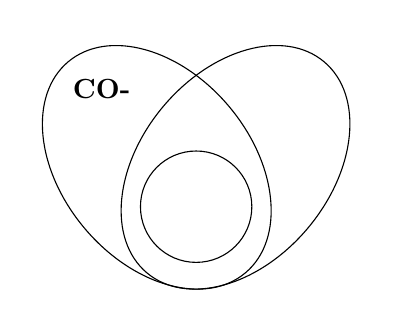
\begin{tikzpicture}
        \node[draw,circle,inner sep=0.5cm] () at (0,0) {$\PClass$};
        \draw (0.5,0.5) ellipse [x radius=1.2cm,y radius=1.75cm,rotate=-40];
        \draw (-0.5,0.5) ellipse [x radius=1.2cm,y radius=1.75cm,rotate=40];
        \node () at (-1.2,1.5) {$\textbf{CO-}\NPClass$};
        \node () at (1.5,1.5) {$\NPClass$};
    \end{tikzpicture}
\end{document}
